\documentclass[12pt,letterpaper]{hmcpset}
\usepackage[margin=1in]{geometry}
\usepackage{graphicx}
\usepackage{amsmath,amssymb}
\usepackage{enumerate}

% info for header block in upper right hand corner
\name{}
\class{Physics 24a - Section ---}
\assignment{Non-Inertial Systems and Fictitious Forces}
\duedate{Monday, April 25, 2016}

\begin{document}

\problemlist{9.\{4,5,6,12\}}

\textbf{Reading} Chapter 9 on non-inertial sytems and fictitious forces. I
will be leaving for Minnesota on Wednesday afternoon, so there will be
no class on Thursday.

\begin{problem}[Weight on a car's wheels - KK 9.4]
    The center of mass of a $1600$kg car is midway between the wheels and
    $0.7$m above the ground. The wheels are $2.6$m apart.
    \begin{enumerate}[a)]
        \item What is the minimum acceleration $A$ of the car so that the front
            wheel just begin to lift off the ground?
        \item If the car decelerates at rate $g$, what is the normal force on the
            front wheels and on the rear wheels?
    \end{enumerate}
\end{problem}
\begin{solution}
    \vfill
\end{solution}
\clearpage

\begin{problem}[Gyroscope and acceleration - KK 9.5]
    Gyroscopes can be used to detect acceleration and measure speed. Consider a
    gyroscope spinning at high speed $\omega_{s}$. The gyroscope is attached to a
    vehicle by a universal pivot $P$. If the vehicle accelerates in the direction
    perpendicular to the spin axis at rate $a$, then the gyroscope will precess
    about the acceleration axis, as shown in the sketch. The total angle of
    precession, $\theta$, is measured.

    Show that if the system starts from rest, the velocity of the vehicle is given
    by 
    \begin{equation*}
        v = \frac{I_{s} \omega_{s}}{M l} \theta
    \end{equation*}
    where $I_{s}\omega_{s}$ is the gyroscope's spin angular momentum, $M$ is the
    total mass of the pivoted portion of the gyroscope, and $l$ is the distance from
    the pivot to the center of mass. (Such a system is called an integrating gyro,
    since it automatically integrates the acceleration to give the velocity.)

    \begin{center}
        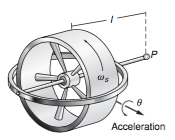
\includegraphics[width=2in]{img/9_5}
    \end{center}
\end{problem}
\begin{solution}
    \vfill
\end{solution}
\clearpage

\begin{problem}[Spinning top in an elevator - KK 9.6]
    A top of mass $M$ spins with angular speed $\omega_{s}$ about its axis, as
    shown. The moment of inertia of the top about the spin axis is $I_{0}$, and
    the center of mass of the top is a distance $l$ from the point. The axis is
    inclined at angle $\phi$ with respect to the vertical, and the top is
    undergoing uniform precession. Gravity is directed downward.

    The top is in an elevator, with its tip held to the elevator floor by a
    frictionless pivot. Find the rate of precession, $\Omega$, clearly indicating
    its direction, in each of the following cases:
    \begin{enumerate}[a)]
        \item The elevator at rest.
        \item The elevator accelerating down at rate $2g$.
    \end{enumerate}

    \begin{center}
        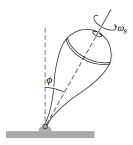
\includegraphics[width=2in]{img/9_6}
    \end{center}
\end{problem}
\begin{solution}
    \vfill
\end{solution}
\clearpage

\begin{problem}[Pendulum on rotating platform - KK 9.12]
    A pendulum is rigidly fixed to an axle held by two supports so that it can
    swing only in a plane perpendicular to the axle. The pendulum consists of a
    mass $M$ attached to a massless rod of length $l$. The supports are mounted on
    a platform that rotates with constant angular velocity $\Omega$. Find the
    pendulum's frequency assuming that the amplitude is small.

    \begin{center}
        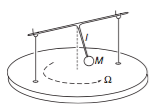
\includegraphics[width=2in]{img/9_12}
    \end{center}
\end{problem}
\begin{solution}
    \vfill
\end{solution}
\clearpage

\end{document}
